%\documentclass[convert={density=300,size=1080x800,outext=.png}]{standalone}
\documentclass{standalone}
\usepackage{tikz}
\usetikzlibrary{decorations.markings}
\usetikzlibrary{arrows}
\usetikzlibrary{patterns}
\newcommand{\xval}{8.5}


\begin{document}

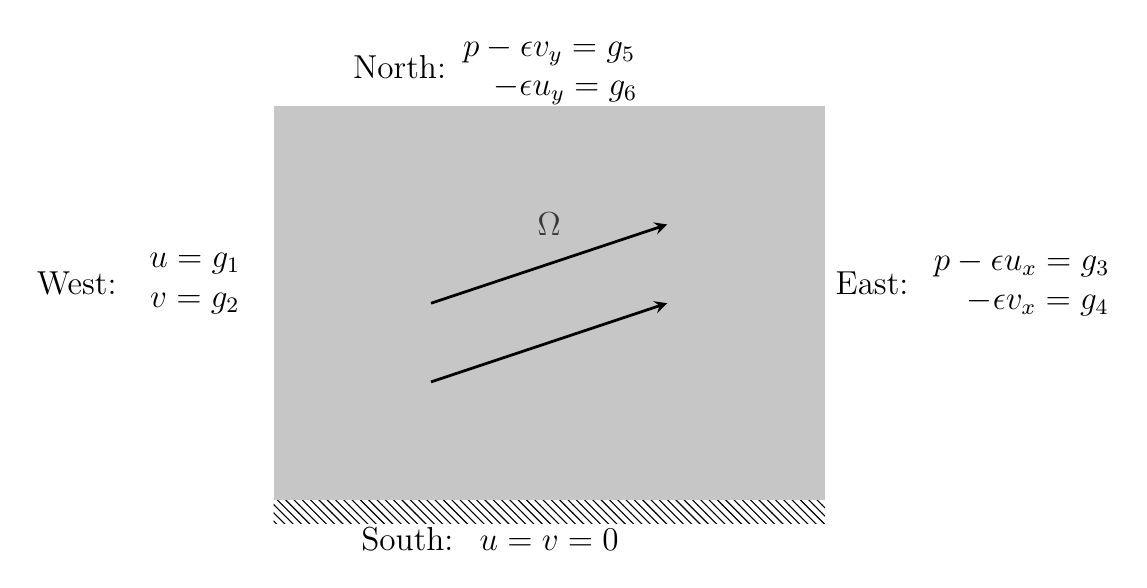
\begin{tikzpicture}%[scale=1.0]
  % background grid for orientation (also gives a better shape to standalone plot)
 %\draw[step=1.0,black,very thin] (-3,-1) grid (7,7);
  
  
  \draw (2.5,3.5) node {{\large $\Omega$}}; 
  
   \draw (-3.5,2.75) node {{\large West:}};
    \draw (-2,3) node {{\large $u = g_1$}};
    \draw (-2,2.5) node {{\large $v = g_2$}};
    \fill[gray,opacity=0.45] (-1,0) -- (6,0) -- (6,5) -- (-1,5) -- cycle;
    
    \draw[->,>=stealth, line width = 1pt] (1,2.5) -- (4,3.5);
    \draw[->,>=stealth, line width = 1pt] (1,1.5) -- (4,2.5);
    
    \fill[pattern=north west lines] (-1,-0.3) rectangle ++(7,0.3);
   \draw (0.7,-0.5) node {{\large South:}};
   \draw (2.5,-0.5) node {{\large $u = v = 0$}};
   \draw (0.6,5.5) node {{\large North:}};
   \draw (2.5,5.7) node {{\large $p-\epsilon v_y = g_5$}};
   \draw (2.5,5.2) node {{\large $\ \  \ -\epsilon u_y = g_6$}};
    
    \draw (6.6,2.75) node {{\large East:}};
    \draw (8.5,3) node {{\large $p - \epsilon u_x = g_3$}};
    \draw (8.5,2.5) node {{\large $\quad - \epsilon v_x = g_4$}};


\end{tikzpicture}

\end{document}
